
The Cyber Security Analytics Framework\cite{Abraham_2016} is a modular process for evaluating system security. CSAF provides a suite of metrics designed to measure facets of system integrity, providing a means of quantitative comparison that directly lends itself to system migration planning. The process follows the basic \textit{input-process-output} sequence established in the \textit{Multi-host, Multi-stage Vulnerability Analysis Language}\cite{Ou_Appel_2005} toolkit MulVal.

\begin{figure}[H]
\centering
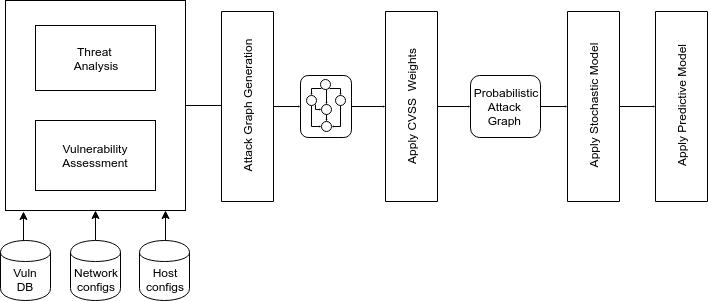
\includegraphics[width=140mm]{resource/img/ch_background/sdn_analytics/CSAF_arch.png}
\caption{Cyber Security Analytics Framework\cite{Abraham_2016}}
\label{fig:csaf_framework}
\end{figure} 

MulVal provides an efficient\cite{Rao_1997} Datalog based modeling language and inference engine for vulnerability relationship analysis. The input model consists of configurations for \textbf{hosts} and \textbf{networks}, \textbf{principals} describing user accounts and privileges, rules governing \textbf{interactions}, and access \textbf{policies}. Information about the system under test is either gathered through standard methods\cite{Ou_Govindavajhala_Appel} such as Nessus, Nmap, and OVAL scans or defined manually for hypothetical data points, and parsed into the global system model using an appropriate adaptor. MulVal can then make inferences about how the entities are able to interact. When provided with a starting and ending node, MulVal enumerates all possible paths an attacker may traverse to compromise the target. The attack graph represents the exploitable vulnerabilities in a system as the set of connected nodes and edges between an attacker’s origin and the target.

Once the attack graph has been generated, the processing stages of the CSAF collect known vulnerabilities, apply weights to the enumerated attack paths, run simulations, and compute analytical measurements for the set of security metrics desired. These measurements are reported for each state model to provide a clear view of system security along a migration path, or to support comparison between competing target systems. The remainder of this section will describe these steps in more detail. %Our methodology can be summarised in the following steps:

% \begin{itemize}
% \item Model the system or network 
% \item Identify threats and vulnerabilities within that network  
% \item Create an attack graph 
% \item Generate stochastic models to simulate attacks
% \item Measure security against derived metrics
% \item Repeat for each distinct state under analysis
% \end{itemize}


